\documentclass[openany]{book}

\usepackage[margin=1in]{geometry}
\usepackage{amsmath,amsfonts,amsthm, amssymb}
\usepackage{yhmath}
\usepackage{mathrsfs}
\usepackage{mathtools}
\usepackage{xcolor}
\usepackage{graphicx}
\usepackage{comment}
\usepackage{tikz-cd}
\usepackage{quiver}
\renewcommand{\familydefault}{ppl}
\newcommand{\R}{\mathbb{R}}
\newcommand{\E}{\mathbb{E}}
\newcommand{\Z}{\mathbb{Z}}
\newcommand{\CC}{\mathcal{C}}
\newcommand{\F}{\mathbb{F}}
\newcommand{\la}{\langle}
\newcommand{\ra}{\rangle}
\newcommand{\colim}{\text{colim}}
\DeclareMathOperator{\im}{im}
\let\oldemptyset\emptyset
\let\emptyset\varnothing
\newcommand{\tor}{\text{Tor}}
\newcommand{\id}{\text{id}}



\usepackage{thmtools,thm-restate}

% Fixing mdframed skip below
% See https://tex.stackexchange.com/a/292090/143086
\usepackage[framemethod=TikZ]{mdframed}
\usepackage{xpatch}
\makeatletter
\xpatchcmd{\endmdframed}
	{\aftergroup\endmdf@trivlist\color@endgroup}
	{\endmdf@trivlist\color@endgroup\@doendpe}
	{}{}
\makeatother

\definecolor{huilightpink}{HTML}{fff2fe}
\definecolor{huidarkpink}{HTML}{d955b7}
\declaretheoremstyle[
	mdframed={
		backgroundcolor=huilightpink,
		linecolor=huidarkpink,
		rightline=false,
		topline=false,
		bottomline=false,
		linewidth=2pt,
		innertopmargin=5pt,
		innerbottommargin=8pt,
		innerleftmargin=8pt,
		leftmargin=-2pt,
		skipbelow=2pt,
		nobreak
	},
	headfont=\normalfont\bfseries\color{huidarkpink}
]{huipinkbox}
\declaretheorem[style=huipinkbox,name=Theorem,within=chapter]{thm}
\declaretheorem[style=huipinkbox,name=Theorem,sibling=thm]{theorem}




\begin{comment}
\definecolor{huilightyellow}{HTML}{fff5d6}
\definecolor{huidarkyellow}{HTML}{fcad03}
\declaretheoremstyle[
	mdframed={
		backgroundcolor=huilightyellow,
		linecolor=huidarkyellow,
		rightline=false,
		topline=false,
		bottomline=false,
		linewidth=2pt,
		innertopmargin=5pt,
		innerbottommargin=8pt,
		innerleftmargin=8pt,
		leftmargin=-2pt,
		skipbelow=2pt,
		nobreak
	},
	headfont=\normalfont\bfseries\color{huidarkyellow}
]{huiyellowbox}
\declaretheorem[style=huiyellowbox,name=Proposition,within=chapter]{prop}
\end{comment}



\definecolor{huilightpurple}{HTML}{faf2ff}
\definecolor{huidarkpurple}{HTML}{912ed9}
\declaretheoremstyle[
	mdframed={
		backgroundcolor=huilightpurple,
		linecolor=huidarkpurple,
		rightline=false,
		topline=false,
		bottomline=false,
		linewidth=2pt,
		innertopmargin=5pt,
		innerbottommargin=8pt,
		innerleftmargin=8pt,
		leftmargin=-2pt,
		skipbelow=2pt,
		nobreak
	},
	headfont=\normalfont\bfseries\color{huidarkpurple}
]{huipurplebox}
\declaretheorem[style=huipurplebox,name=Proposition,within=chapter]{prop}



% \definecolor{huilightpurple}{HTML}{faf2ff}
% \definecolor{huidarkpurple}{HTML}{912ed9}
% \declaretheoremstyle[
% 	mdframed={
% 		backgroundcolor=huilightpurple,
% 		linecolor=huidarkpurple,
% 		rightline=false,
% 		topline=false,
% 		bottomline=false,
% 		linewidth=2pt,
% 		innertopmargin=5pt,
% 		innerbottommargin=8pt,
% 		innerleftmargin=8pt,
% 		leftmargin=-2pt,
% 		skipbelow=2pt,
% 		nobreak
% 	},
% 	headfont=\normalfont\bfseries\color{huidarkpurple}
% ]{huipurplebox}
\declaretheorem[style=huipurplebox,name=Lemma,within=chapter]{lem}


\definecolor{lightpink}{HTML}{f0f6fc}
\definecolor{darkpink}{HTML}{2c72b8}
\declaretheoremstyle[
	mdframed={
		backgroundcolor=lightpink,
		linecolor=darkpink,
		rightline=false,
		topline=false,
		bottomline=false,
		linewidth=2pt,
		innertopmargin=5pt,
		innerbottommargin=8pt,
		innerleftmargin=8pt,
		leftmargin=-2pt,
		skipbelow=2pt,
		nobreak
	},
	headfont=\normalfont\bfseries\color{darkpink}
]{pinkbox}
\declaretheorem[style=pinkbox,name=Definition,within=chapter]{defn}


\definecolor{huilightblue}{HTML}{edf9ff}
\definecolor{huidarkblue}{HTML}{4b79db}
\declaretheoremstyle[
	mdframed={
		backgroundcolor=huilightblue,
		linecolor=huidarkblue,
		rightline=false,
		topline=false,
		bottomline=false,
		linewidth=2pt,
		innertopmargin=5pt,
		innerbottommargin=8pt,
		innerleftmargin=8pt,
		leftmargin=-2pt,
		skipbelow=2pt,
		nobreak
	},
	headfont=\normalfont\bfseries\color{huidarkblue}
]{huiblueblox}
\declaretheorem[style=huiblueblox,name=Example,within=chapter]{example}



% \definecolor{huilightblue}{HTML}{edf9ff}
% \definecolor{huidarkblue}{HTML}{4b79db}
% \declaretheoremstyle[
% 	mdframed={
% 		backgroundcolor=huilightblue,
% 		linecolor=huidarkblue,
% 		rightline=false,
% 		topline=false,
% 		bottomline=false,
% 		linewidth=2pt,
% 		innertopmargin=5pt,
% 		innerbottommargin=8pt,
% 		innerleftmargin=8pt,
% 		leftmargin=-2pt,
% 		skipbelow=2pt,
% 		nobreak
% 	},
% 	headfont=\normalfont\bfseries\color{huidarkblue}
% ]{huiblueblox}
% \declaretheorem[style=huiblueblox,name=Example,within=chapter]{example}

% \declaretheoremstyle[
% 	mdframed={
% 		backgroundcolor=huilightblue,
% 		linecolor=huidarkblue,
% 		rightline=false,
% 		topline=false,
% 		bottomline=false,
% 		linewidth=2pt,
% 		innertopmargin=5pt,
% 		innerbottommargin=8pt,
% 		innerleftmargin=8pt,
% 		leftmargin=-2pt,
% 		skipbelow=2pt,
% 		nobreak
% 	},
% 	headfont=\normalfont\bfseries\color{huidarkblue}
% ]{huiblueblox}
\declaretheorem[style=huiblueblox,name=Problem,within=chapter]{prob}



% \declaretheoremstyle[
% 	mdframed={
% 		backgroundcolor=huilightblue,
% 		linecolor=huidarkblue,
% 		rightline=false,
% 		topline=false,
% 		bottomline=false,
% 		linewidth=2pt,
% 		innertopmargin=5pt,
% 		innerbottommargin=8pt,
% 		innerleftmargin=8pt,
% 		leftmargin=-2pt,
% 		skipbelow=2pt,
% 		nobreak
% 	},
% 	headfont=\normalfont\bfseries\color{huidarkblue}
% ]{huiblueblox}
\declaretheorem[style=huiblueblox,name=Exercise,within=chapter]{exer}
\declaretheorem[style=huipinkbox, name=Corollary, within=chapter]{cor}





















\newcommand{\nirwarnsymbol}{%
	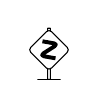
\begin{tikzpicture}[baseline=(x.base)]
		\draw[rounded corners=.01em] (-.05em,-1.07em)rectangle(.05em,.78em);
		\draw[fill=white,rounded corners=1.3] (0,.75em)--(.75em,0)--(0,-.75em)--(-.75em,0)--cycle;
		\draw[line width=0.2mm, line cap=round](-.4em,-1.07em)--(.4em,-1.07em);
		\node(x) at (0,0em) {};
		% Thank you https://tex.stackexchange.com/a/262510
		\draw[
			line cap=but,
			line join=round,
			x=.5em,
			line width=0.5mm,
			y=1*(height("Z")-\pgflinewidth)*(1-sin(10)),
			rotate=-10,
			rounded corners=1.5pt,
		](-0.57, 0.57) -- (0.57, 0.57) -- (-0.57, -0.57) -- (0.57, -0.57);
	\end{tikzpicture}%
}

%%%%%%%%%%%%%%%%%%%%%%%%%%%%%%%%%%%%%%%%%%%% MARGINS
\usepackage{marginnote}
% Thank you https://tex.stackexchange.com/a/472882
% Makes marginnotes always appear on the left, apparently
%
\makeatletter
\long\def\@mn@@@marginnote[#1]#2[#3]{%
	\begingroup
		\ifmmode\mn@strut\let\@tempa\mn@vadjust\else
			\if@inlabel\leavevmode\fi
			\ifhmode\mn@strut\let\@tempa\mn@vadjust\else\let\@tempa\mn@vlap\fi
		\fi
		\@tempa{%
			\vbox to\z@{%
				\vss
				\@mn@margintest
				\if@reversemargin\if@tempswa
						\@tempswafalse
					\else
						\@tempswatrue
				\fi\fi

					\llap{%
						\vbox to\z@{\kern\marginnotevadjust\kern #3
							\vbox to\z@{%
								\hsize\marginparwidth
								\linewidth\hsize
								\kern-\parskip
								%\mn@parboxrestore
								\marginfont\raggedleftmarginnote\strut\hspace{\z@}%
								\ignorespaces#1\endgraf
								\vss
							}%
							\vss
						}%
						\if@mn@verbose
							\PackageInfo{marginnote}{xpos seems to be \@mn@currxpos}%
						\fi
						\begingroup
							\ifx\@mn@currxpos\relax\else\ifx\@mn@currpos\@empty\else
									\kern\@mn@currxpos
							\fi\fi
							\ifx\@mn@currpage\relax
								\let\@mn@currpage\@ne
							\fi
							\if@twoside\ifodd\@mn@currpage\relax
									\kern-\oddsidemargin
								\else
									\kern-\evensidemargin
								\fi
							\else
								\kern-\oddsidemargin
							\fi
							\kern-1in
						\endgroup
						\kern\marginparsep
					}%
			}%
		}%
	\endgroup
}
\makeatother
%
% Mostly for todonotes
\renewcommand{\marginpar}{\marginnote}
%%%%%%%%%%%%%%%%%%%%%%%%%%%%%%%%%%%%%%%%%%%% /MARGINS

\definecolor{nirlightred}{RGB}{250, 220, 220}
\definecolor{nirdarkred}{HTML}{f40000}
\declaretheoremstyle[
	mdframed={
		backgroundcolor=nirlightred,
		linecolor=nirdarkred,
		rightline=false,
		topline=false,
		bottomline=false,
		linewidth=2pt,
		innertopmargin=5pt,
		innerbottommargin=8pt,
		innerleftmargin=8pt,
		leftmargin=-2pt,
		skipbelow=2pt,
		nobreak
	},
	headfont=\normalfont\bfseries\color{nirdarkred}
]{nirredbox}

% \makeatletter
% \declaretheorem[
% 	style=nirredbox,
% 	name=Warning,
% 	sibling=thm,
% 	% without \leavevmode, the first item in a list gets misformatted
% 	postheadhook={\leavevmode\marginnote{\nirwarnsymbol}[-3pt]%
% 	\ifthmt@thisistheone% restatable makes alignment weird
% 		\hspace{-2.2pt}%
% 	\fi}
% ]{warn}
% \makeatother

\newcommand{\nirideasymbol}{%
	
\begin{tikzpicture}[baseline=(x.base)]
		\draw[rounded corners=.01em] (-.05em,-1.07em)rectangle(.05em,.78em);
		\draw[fill=white,rounded corners=1.3] (0,.75em)--(.75em,0)--(0,-.75em)--(-.75em,0)--cycle;
		\draw[line width=0.2mm, line cap=round](-.4em,-1.07em)--(.4em,-1.07em);
		\node(x) at (0,0em) {};
		\node at (0,0em) {{\textbf{!}}};
	\end{tikzpicture}%
}
\renewcommand{\nirwarnsymbol}{%
	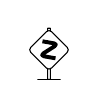
\begin{tikzpicture}[baseline=(x.base)]
		\draw[rounded corners=.01em] (-.05em,-1.07em)rectangle(.05em,.78em);
		\draw[fill=white,rounded corners=1.3] (0,.75em)--(.75em,0)--(0,-.75em)--(-.75em,0)--cycle;
		\draw[line width=0.2mm, line cap=round](-.4em,-1.07em)--(.4em,-1.07em);
		\node(x) at (0,0em) {};
		% Thank you https://tex.stackexchange.com/a/262510
		\draw[
			line cap=but,
			line join=round,
			x=.5em,
			line width=0.5mm,
			y=1*(height("Z")-\pgflinewidth)*(1-sin(10)),
			rotate=-10,
			rounded corners=1.5pt,
		](-0.57, 0.57) -- (0.57, 0.57) -- (-0.57, -0.57) -- (0.57, -0.57);
	\end{tikzpicture}%
}
\makeatletter
\declaretheorem[
	style=nirredbox,
	name=Idea,
	sibling=thm,
	% without \leavevmode, the first item in a list gets misformatted
	postheadhook={\leavevmode\marginnote{\nirideasymbol}[-3pt]%
	\ifthmt@thisistheone% restatable makes alignment weird
		\hspace{-2.2pt}%
	\fi}
]{idea}

\declaretheorem[
	style=nirredbox,
	name=Warning,
	sibling=thm,
	% without \leavevmode, the first item in a list gets misformatted
	postheadhook={\leavevmode\marginnote{\nirwarnsymbol}[-3pt]%
	\ifthmt@thisistheone% restatable makes alignment weird
		\hspace{-2.2pt}%
	\fi}
]{warn}
\makeatother

\title{Algebraic Topology}

\date{\today}
\author{Hui Sun}

\begin{document}

\maketitle

\tableofcontents



\newpage

\chapter{Category Theory}
\textbf{Instructor:} Nitu Kitchro, 
\textbf{Office Hours}: Monday after class, \textbf{TA: } Anna Matsui
\section{Lecture 1 8/26}
\begin{defn}[Category]
    A category $\mathcal{C}$ consists of the following data:
    \begin{enumerate}
        \item A collection of objects denoted as Ob$(\mathcal{C})$
        \item Given two objects $X,Y\in$ Ob$(\mathcal{C})$, a collection of morphisms between $X,Y$, $f:X\to Y$, denoted as mor$_\CC(X,Y)$.
        \item (Composition) We have mor$_\CC(X,Y)\times mor_\CC(Y,Z)\to mor_\CC(X,Z)$ that satisfies associativity
        \begin{equation*}
            f\circ(g\circ h)=(f\circ g)\circ h
        \end{equation*}
        \item (Identity) There is a distinguished morphism for each $X$, $Id_\CC(X,X)$ such that given any $f\in mor(X,Y)$, we have $f\circ id_X=id_Y\circ f=f$.
    \end{enumerate}
\end{defn}
In this course, we will make the assumption that in all the categories that we work with, Ob$(\CC)$ need not be a set, but given any $X,Y\in Ob(\CC)$, mor$(X,Y)$ will always be a set. Now we talka bout some examples of categories.
\begin{example}[Sets]
    Let Ob$(Sets)$ be all the sets in the universe. Given $X,Y$ sets, mor$(X,Y)$ be all the set maps from $X$ to $Y$, and $id_X$ is the identity map.
\end{example}
\begin{example}[Top]
    Let Ob$(Top)$ be all the topological spaces, and mor$(X,Y)$ be all the continuous maps from $X$ to $Y$.
\end{example}
\begin{example}[Vect$_\F$]
    Let $\F$ be a field, and let Ob be all the $\F$-vector spaces. Then mor$(V,W)$ is all the $\F$-linear homomorphisms from $V$ to $W$, where $id_V$ is the identity homomorphism.
\end{example}
\begin{example}[Posets]
    Fix a poset $P$, let Ob$(P)$ be the collection of elements in $P$, and given $p,q$ we define 
    \begin{equation*}
        mor(p,q)=\begin{cases}
            *, \text{ if } q\leq p\\
            \emptyset, \text{ otherwise }
        \end{cases}
    \end{equation*}
\end{example}
\begin{prob}
    \textbf{HW(Q1): check this is a category}
\end{prob}
\begin{example}[Opposite category]
    Given a category $\CC$, there is another category called the opposite category, denoted as $\CC^{op}$, where 
    \begin{enumerate}
        \item The objects are the same as $\CC$
        \item Given $X,Y\in$ Ob$(C^{op})$, we have mor$_{op}(X,Y):=$ mor$_\CC(Y,X)$. 
        \item Moreover, given $f\in mor_{op}(X,Y), g\in mor_{op}(Y,Z)$, then $g\circ f$ in $C^{op}$ is $f\circ g: Z\to X$.
    \end{enumerate}
\end{example}
Naturally, we define isomorphisms now.
\begin{defn}[isomorphism]
    Given a category $\CC$, and a morphism $f\in mor_C(X,Y)$, we say $f$ is an isomorphism if there exists $g\in mor_C(Y,X)$ such that 
    \begin{equation*}
        f\circ g=Id_Y, g\circ f=Id_X
    \end{equation*}
\end{defn}
Now we introduce maps between categories.
\begin{defn}[functor]
    Given categories $\CC,\mathcal{D}$, a functor $F:C\to D$ is the following;
    \begin{enumerate}
        \item Given an object $X$ in $\mathcal{C}$, $F(X)$ is an object in $D$. 
        \item Given a morphism $f: X\to Y$, $F(f)$ is a functor $F(f): F(X)\to F(Y)$. Moreover, it satisfies the following:
        \begin{enumerate}
            \item $F(id_X)=id_{F(X)}$
            \item $F(f\circ g)=F(f)\circ F(g)$. Alternatively, we can rewrite this condition as the following: 
            \[\begin{tikzcd}
                {mor(X,Y)\times mor(Y,Z)} & {mor(X,Z)} \\
                {mor(F(X), F(Y))\times mor(F(Y),F(Z))} & {mor(F(X),F(Z))}
                \arrow[from=1-1, to=1-2]
                \arrow["{mor(F)\times mor(F)}", from=1-1, to=2-1]
                \arrow["{mor(F)}", from=1-2, to=2-2]
                \arrow[from=2-1, to=2-2]
            \end{tikzcd}\]
            such that this diagram commutes.
        \end{enumerate}
    \end{enumerate}
\end{defn}
\begin{prob}
    \textbf{HW(Q2): functors take isomorphisms to isomorphisms.}
\end{prob}
Now we talk about some examples of functors.
\begin{example}
    $F: Top\to Set$, where $X\mapsto X$, where the latter is a set, and $f\mapsto f$ as set maps.
\end{example}
\begin{example}
    Let $\F$ be a field, and $F: Sets\to \text{Vect}_\F$, where $X\mapsto \F\la X\ra$, where $\F\la X\ra$ is the free vector space over $\F$ on the set $X$.
\end{example}
\begin{prob}
    \textbf{HW(Q3): extend this to a functor by defining $mor(f)$ and show this is a functor.}
\end{prob}
\begin{example}
    Let $\F$ be a field, then the following is a functor, $F: Sets^{op}\to\text{Vect}_\F$, where
    \begin{equation*}
        h  F: X\mapsto Maps(X,\F)
    \end{equation*}
\end{example}
\begin{prob}
    \textbf{HW(Q4)}: show this extends to a functor by defining $F(f)$, and show it is a functor.
\end{prob}

\section{Lecture 2 8/28}
\begin{defn}[contravariant functor]
    Let $F:\CC\to\mathcal{D}$ is a contravariant functor from $\CC^{op}\to\mathcal{D}$, (equivalently, $\CC\to\mathcal{D}^{op}$).
\end{defn}
\begin{prob}
    \textbf{HW(Q5):} Show that the following functor $F$ from Vect$_\F$ to Vect$_\F$ extends to a contravariant functor, where 
    \begin{equation*}
        Ob_F: V\mapsto V^*=Hom(V,\F)
    \end{equation*}
    i.e., define the morphism function and show it is a contravariant functor.
\end{prob}
We remark that we can define a category of categories: let $Cat$ be the category of categories, with morphisms as functors, and note that objects or morphisms in this case are both not sets!
\begin{defn}[natural transformation]
    Given functors $F,G: \CC\to\mathcal{D}$, a natural transformation $T$ from $F$ to $G$ is the following: $T: F\Rightarrow G$:
    \begin{enumerate}
        \item given object $X\in Ob(\CC)$, $T(X)\in mor(F(X),G(X))$
        \item Given $f\in mor(X,Y)$, the following diagram commutes:
        \[\begin{tikzcd}
            {F(X)} & {F(Y)} \\
            {G(X)} & {G(Y)}
            \arrow["{F(f)}", from=1-1, to=1-2]
            \arrow["{T(X)}"', from=1-1, to=2-1]
            \arrow["{T(Y)}", from=1-2, to=2-2]
            \arrow["{G(f)}"', from=2-1, to=2-2]
        \end{tikzcd}\]
        where $mor_F, mor_G$ is the identification function on morphisms by functors $F,G$
    \end{enumerate}
    If for all $X$, $T(X)$ is an isomorphism, then this natural transformation is called a natural isomorphism.
\end{defn}
In other words, this natural transformation is how one takes a functor $F$ and turn it to another functor $G$. We will (in a homework) show there exists natural transofrmation between the following two functors.
\begin{example}
    Consider $F,G: Vect_\F\to Vect_\F$, define 
    \begin{equation*}
        F(V)=V\otimes_\F V/_{\la a\otimes b-b\otimes a\ra}=V\otimes_\F V/\Sigma_2, G(V)=(V\otimes_F V)^{\Sigma_2}=\{\alpha\in V\otimes_\F V: \sigma(\alpha)=\alpha\}
    \end{equation*}
    Both are vector spaces are fixed under ``swaps.'' Then a natural transformation can be defined as follows $T(V):$
    \begin{equation*}
        T(V): a\otimes b\mapsto a\otimes b+b\otimes a
    \end{equation*}
\end{example}
\begin{prob}
    \textbf{HW(Q6):} For the above $F,G$
    \begin{enumerate}
        \item Show that $T$ defines a natural transformation from $F$ to $G$. 
        \item Find conditions on $\F$ for $T$ being a natural isomorphism.
    \end{enumerate}
\end{prob}
Next we define limits and colimits.
    Let $\mathcal{C},\mathcal{D}$ be categories, $d$ be an object in $\mathcal{D}$, then we can define a functor $F_d: \mathcal{C}\to\mathcal{D}$ such that for any object $c$ in $\mathcal{C}$,
    \begin{equation*}
        F_d(c)=d, F_d(f)=Id_d
    \end{equation*}
    In other words, this is the ``constant functor'' on $\mathcal{D}$, i.e., every object is sent to $d$, and every morphism is sent to $id_d$.
\begin{defn}[colimit]
    Given any functor $F:\mathcal{C}\to\mathcal{D}$, the colimit of $F$, denoted as $\colim(F)$ is an object in $\mathcal{D}$ endowed with a natural transformation:
    \begin{equation*}
        \varphi_F:F\Rightarrow F_{\colim(F)}
    \end{equation*}
    such that given any other object $d$ in $D$ and a natural transformation 
    \begin{equation*}
        \varphi: F\Rightarrow F_d
    \end{equation*}
    there exists a unique morphism in $\mathcal{D}$, $f:\colim(F)\to d$ making the following diagram commute: for any $X,Y,g$:
    \[\begin{tikzcd}
        {F(X)} && {F(Y)} \\
        & {\text{colim}(F)} \\
        & d
        \arrow["{F(g)}", from=1-1, to=1-3]
        \arrow["{\varphi_F}", from=1-1, to=2-2]
        \arrow["\varphi"', curve={height=12pt}, from=1-1, to=3-2]
        \arrow["{\varphi_F}"', from=1-3, to=2-2]
        \arrow["\varphi", curve={height=-12pt}, from=1-3, to=3-2]
        \arrow["{\textcolor{red}{f}}", from=2-2, to=3-2]
    \end{tikzcd}\]
\end{defn}
Next we prove some facts about colimits and give an example, where $\colim(F)$ exists.
\begin{prop}
    If $\colim F$ exists, then $\colim F$ is unique up to isomorphisms.
\end{prop}
\begin{proof}
    Let $\colim(F), \colim(F)'$ be two colimits that satisfy the criteria. They are both objects in $\mathcal{D}$, then we get a morphism $f:\colim(F)\to\colim(F)'$, and likewise $g:\colim(F)\to\colim(G)'$, then
    \begin{equation*}
        f\circ g:\colim(F)'\to\colim(F)'
    \end{equation*} 
    is the only morphism, and is the identity morphism. Similarly for $g\circ f$.
\end{proof}
Next we demonstrate a fact via an example.
\begin{thm}
    Let $\mathcal{C}$ be a category where $Ob(\mathcal{C}), mor(X,Y)$ are all sets. Let $F: \mathcal{C}\to\text{Top}$ be any functor, then $\colim(F)$ exists.
\end{thm}
\begin{proof}
    Define $\colim(F):=\bigsqcup_{c}F(c)/\sim$, where $\sim$ is induced by the equivalence relation given by 
    \begin{equation*}
        y\sim F(f)y
    \end{equation*}
    where $y\in F(C_1), f:C_1\to C_2, F(f)x\in F(C_2)$. The natural transformation we endow on $F$ as $\varphi_F:F\Rightarrow F_{\colim(F)}$:
    \begin{equation*}
        \varphi_F: F(C)\mapsto \bigsqcup_{C\in Ob(C)}F(C)/\sim
    \end{equation*}
\end{proof}
\begin{prob}
    \textbf{HW(Q7):} Show that $\colim(F), \varphi_F$ is indeed a colimit. 
\end{prob}
We note that colimits also exist (the same argument goes through) if we replace $\text{Top}$ with groups, sets, but with slightly different constructions, replacing disjoint unions with products, etc.

\begin{defn}[limit]
    Given a functor $F: \mathcal{C}\to\mathcal{D}$, the limit of $F$, denoted as $\lim(F)$ is an object of $\mathcal{D}$, endowed with a natural transformation:
    \begin{equation*}
        \varphi_F: F_{\lim(F)}\Rightarrow F
    \end{equation*}
    such that given any other object $d\in Ob(\mathcal{D})$ and a natural transformation 
    \begin{equation*}
        \varphi: F_d\to F
    \end{equation*}
    there exists a unique $f: \lim F\to d$ such that the following diagram commutes:
    \[\begin{tikzcd}
        & {\lim F} \\
        & d \\
        {F(X)} && {F(Y)}
        \arrow["{\textcolor{red}{f}}", from=1-2, to=2-2]
        \arrow["{\varphi_F}"', curve={height=12pt}, from=1-2, to=3-1]
        \arrow["{\varphi_F}"', curve={height=-12pt}, from=1-2, to=3-3]
        \arrow["\varphi"', from=2-2, to=3-1]
        \arrow["\varphi", from=2-2, to=3-3]
        \arrow["{F(g)}"', from=3-1, to=3-3]
    \end{tikzcd}\]
\end{defn}
Just like colimits, limits are unique up to isomorphisms. 
\begin{prob}
    \textbf{HW(Q8):} Given $F:\mathcal{C}\to\mathcal{D}$, consider $F^{op}:\mathcal{C}^{op}\to\mathcal{D}^{op}$, then 
    \begin{equation*}
        \lim F=\colim F^{op}
    \end{equation*}
\end{prob}
The above problem is interpretation of diagrams and essentially we just reverse all the maps.

\section{Lecture 3 9/4}
Today we define (co)chain complexes: let $R$ be a commutative ring, let $Mod_R$ denote the category of $R$-modules and $R$-module maps.
\begin{defn}[chain complex]
    A chain complex of $R$-modules is a collection of $R$-modules and $R$-modules maps 
    \begin{equation*}
        \dots\to M_{i+1}\xrightarrow{\partial_{i+1}}M_i\xrightarrow{\partial_i}M_{i-1}\xrightarrow{\partial_{i-1}}\dots
    \end{equation*}
    such that $\partial_i\circ\partial_{i+1}=0$ for all $i$. In other words, the image of previous map is contained in the kernal of the subsequent map. In short, we have 
    \begin{equation*}
        \partial^2=0
    \end{equation*}
    We will denote a chain complex by $\{M.; \partial.^M\}$.
\end{defn}
Next we introduce morphisms between chain complexes.
\begin{defn}[morphism between complexes]
    Let $\{M.;\partial.^M\}, \{N.;\partial.^N\}$, a morphism $\{f.\}$ between chain complexes is a ``ladder'' such that the following commutes:
    \[\begin{tikzcd}
        \dots & {M_{i+1}} & {M_i} & {M_{i-1}} & \dots \\
        \dots & {N_{i+1}} & {N_i} & {N_{i-1}} & \dots
        \arrow[from=1-1, to=1-2]
        \arrow["{\partial_{i+1}^M}", from=1-2, to=1-3]
        \arrow["{\partial_i^M}", from=1-3, to=1-4]
        \arrow[from=1-4, to=1-5]
        \arrow[from=2-1, to=2-2]
        \arrow["{\partial_{i+1}^N}", from=2-2, to=2-3]
        \arrow["{\partial_{i}^N}", from=2-3, to=2-4]
        \arrow[from=2-4, to=2-5]
    \end{tikzcd}\]
    Moreover, we define composition of morphisms:
    \begin{equation*}
        \{f.\}\circ \{g.\}:=\{(f\circ g).\}
    \end{equation*}
    where $\{g.\}:\{M.;\partial.^M\}\to\{N.;\partial.^N\}$, and $\{f.\}:\{N.;\partial.^N\}\to \{L.;\partial.^L\}$, which is simply vertical stacking.
\end{defn}
\begin{prob}
    \textbf{HW(Q9):} Prove that chain complexes of $R$-modules form a category $\text{ch}_R$.
\end{prob}
There are interesting functors $F:\text{ch}_R\to Mod_R$, and we begin with the following one:
\begin{defn}[$H_n$, $n$th-homology]
    Given $n\in\mathbb{Z}$, there is a functor 
    \begin{equation*}
        H_n: \text{ch}_R\to Mod_R
    \end{equation*}
    defined as follows:
    \begin{equation*}
        H_n(\{M.;\partial.^M\}):=\ker\partial_n^M\big/ Im \partial_{n+1}^M
    \end{equation*}
    and for $f:\{M.;\partial.^M\}\to\{N.;\partial.^N\}$, we define: $H_n(f): H_n(\{M.;\partial.^M\})\to H_n(\{N.;\partial.^N\})$,
    \begin{equation*}
        H_n(f)[x]:=[f_n(x)]
    \end{equation*}
    where $[x]\in H_n(\{M.;\partial.^M\})$.
\end{defn}




\end{document}